%% title page
\begin{titlepage}
  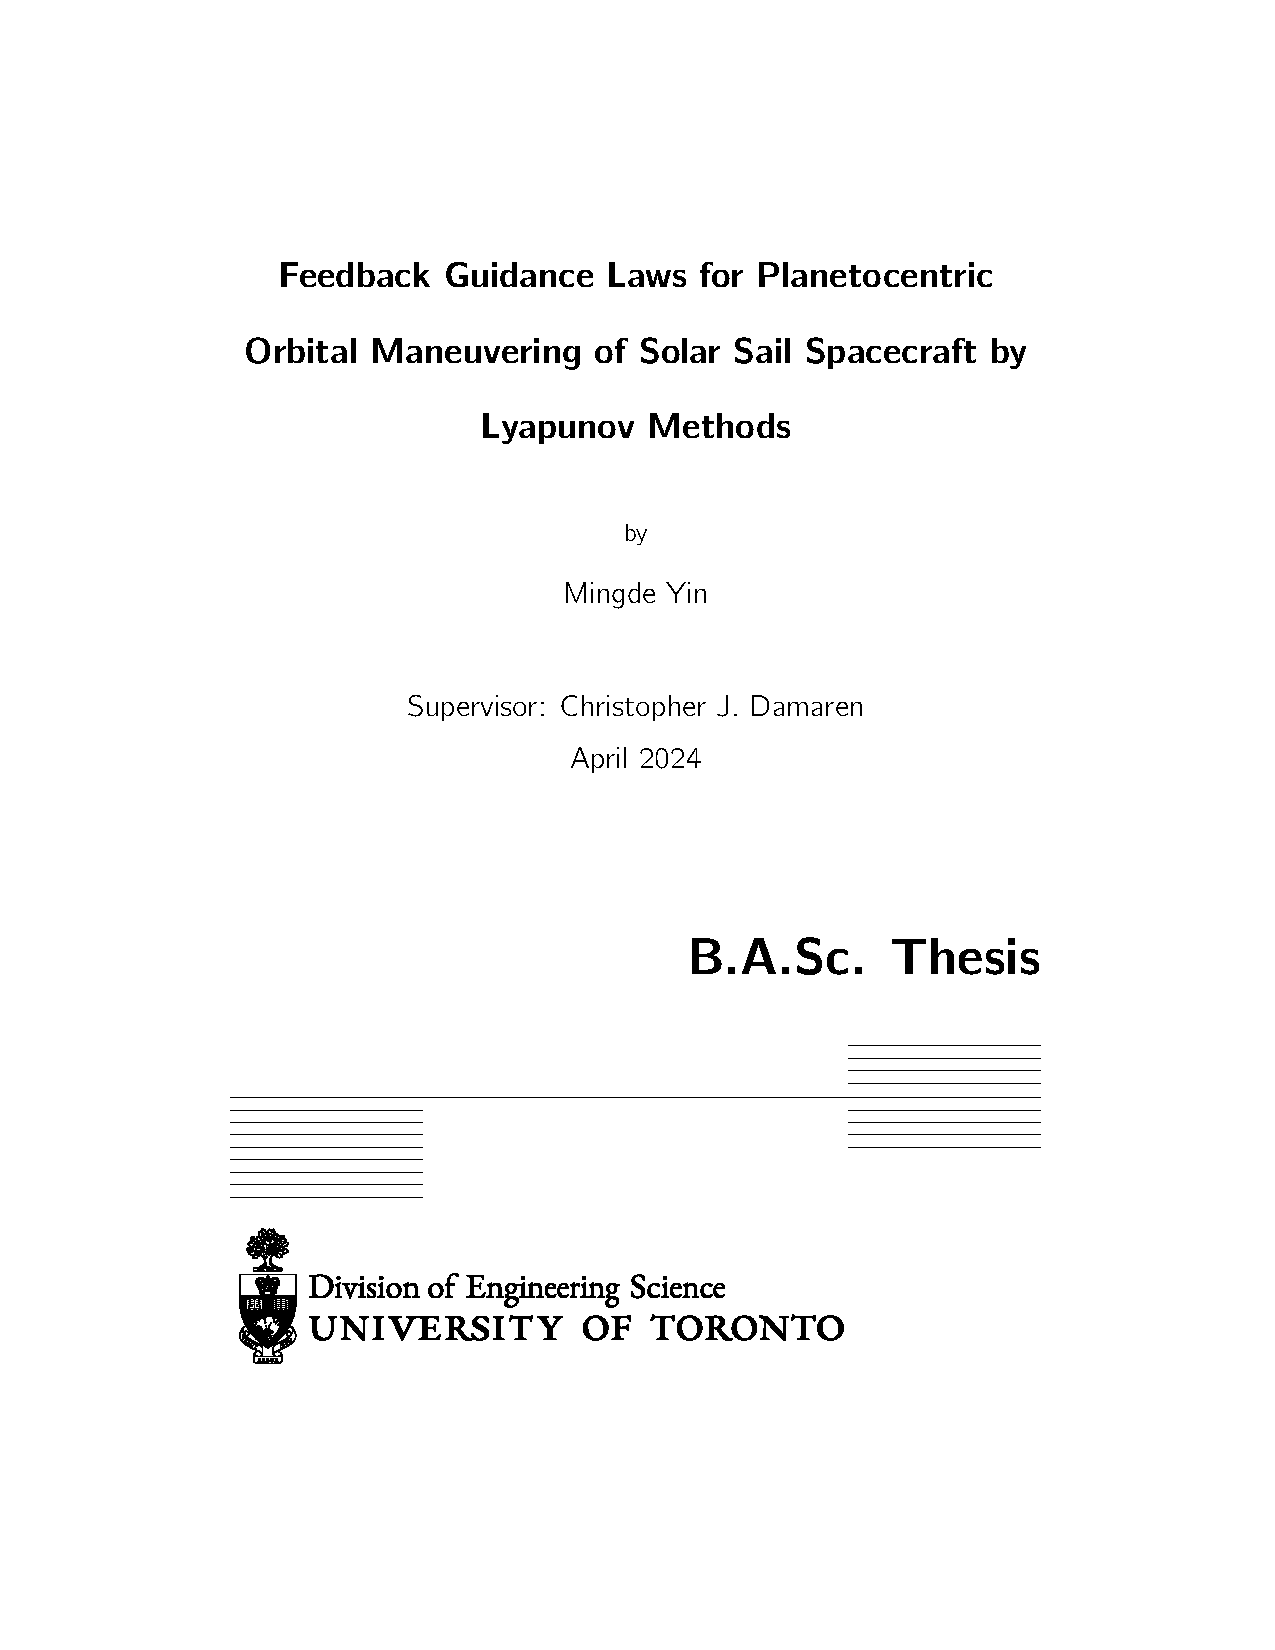
\includepdf{Thesis_Title_Page.pdf}
\end{titlepage}

%% Quote page
\epigraph{
  The cosmos is all that is or ever was or ever will be. Our contemplations of the cosmos stir us. There is a tingling in the spine, a catch in the voice, a faint sensation: as if a distant memory of falling from a great height. We know we are approaching the grandest of mysteries.}{Carl Sagan, \textit{Cosmos}}

\newpage

%% Abstract & Acknowledgements
\vspace*{\fill}
\section*{Abstract}
This thesis develops a guidance law for multi-revolution planetocentric maneuvering of a solar sail spacecraft. QUAIL (\textit{Q-Law} Using Angle of Incidence Limits) adapts the highly successful \textit{Q-Law} from conventional low-thrust guidance. The first stage uses a \textit{Q-Law} formulated in modified equinoctial orbital elements which is agnostic of solar sail dynamics, producing an ``ideal'' thrust direction which is then altered by a heuristic-based second stage to restrict the angle of thrust relative to incident light. Although tampering with the solution produced by the \textit{Q-Law} relaxes the Lyapunov stability of the guidance law, doing so overcomes the challenge of direction-limited thrust availability inherent to solar sail spacecraft flying planetocentric trajectories; sacrificing instantaneous progress towards the target orbit allows the spacecraft to ``wait'' until the Sun is in a better position to perform maneuvers requiring particular thrust directions. QUAIL is tested in simulations on a set of complex orbit-to-orbit transfers, achieving convergence in all cases. An extended study to optimize time of flight is performed using stochastic global optimization of guidance parameters, reducing time of flight up to 30\%. A further set of cases including \(J2\) perturbation demonstrates the robustness of QUAIL against environmental disturbances. Additionally, artificial restriction of the maximum cone angle (for mimicking a real solar sail) is tested, with convergence still achieved under a maximum cone angle of 50 degrees. Overall, the robustness of the underlying \textit{Q-Law} and the minimal dependence on sail characteristics make QUAIL suitable for developing new solar sail dynamics and mission designs.
\vspace*{\fill}

\newpage
\vspace*{\fill}
\section*{Acknowledgements}
I have been incredibly fortunate to work with and learn from a multitude of extraordinarily brilliant minds throughout the richest five years of my life. I would like to thank my supervisor, Professor Christopher Damaren for giving me the opportunity to study this topic and for showing me the awe and beauty of spaceflight. I would like to thank Sanjeev for writing the paper that introduced me to the \textit{Q-Law} and served as the starting point for my understanding of low-thrust spacecraft guidance. I would like to thank my classmates in the Engineering Science program, particularly in the 2T3 Aerospace Engineering cohort for showing me what it means to reach the stars, and for continuously inspiring me to do better. I give particular thanks for Eric, Daniel, Theo, and Rassam for constituting the best capstone teams I could have ever asked for, and for providing the psycho-sociological support I needed to make it here. I would like to thank my course instructors, who, since my first day of EngSci have shaped me into the student I am today. I would also like to thank my high school friends who have kept in touch throughout all these years for sharing with me the rich and enjoyable experiences which have kept me going throughout my undergraduate studies. I would like to thank my parents Xinguo and Yanlu for believing in my dreams of becoming an aerospace engineer, and for all the numerous sacrifices they have undertaken throughout the past twenty three years to afford me the opportunity of realizing my dreams. I would like to thank my sister Connie for showing me a reflection of my own life through growing up, as well as the rest of my family for their encouragements from half a world away.
\vspace*{\fill}


\tableofcontents
\listoffigures
\listoftables